\documentclass{assignment}

\usepackage{float}
\usepackage{tikz}
\usepackage{adjustbox}
\usepackage{titlesec}
\usepackage{soul}
\usepackage{csvsimple}

\usepackage{graphicx}
\usepackage{subcaption}
\usetikzlibrary{shapes, arrows}

\usetikzlibrary{calc,patterns,angles,quotes}
\setlength{\parindent}{0pt}

\hypersetup{
pdftitle={Advanced Dynamics of Mechanical Systems},
pdfsubject={Report for assignment 1},
pdfauthor={Tommaso Bocchietti}
}

\makeglossaries

% \newacronym{cfd}{CFD}{Computational Fluid Dynamics}

\begin{document}

\title{Advanced Dynamics of Mechanical Systems \\ Assignment 1}
\author{Tommaso Bocchietti 10740309 \\ Nome Cognome Codice Persona \\ Nome Cognome Codice Persona}
\date{A.Y. 2023/24}

\maketitle

\begin{figure}[H]
    \centering
    \includegraphics[width=0.7\textwidth]{./pdf/Polimi_logo_coverpage.pdf}
    \label{fig:Polimi_logo}
\end{figure}

\clearpage
\tableofcontents
\listoffigures
\listoftables
% \lstlistoflistings
% \printglossary[type=\acronymtype]

\clearpage
\section{Requests (Part A)}
\label{sec:requests_part_A}

The requests for `Assignment 1 (Part A)' are the followings:

\begin{itemize}
    \item Briefly describe the procedure followed for computing natural frequencies and mode shapes. Plot the mode shapes of the first four modes with the indication of the associated natural frequencies and provide comments to the results.
    \item Compute the FRFs for some combinations of input and output positions. Comment the results.
    \item Briefly describe the procedure followed for identifying the natural frequencies, damping ratios and mode shapes of the first four modes, relying on the FRF-based multi-mode curve fitting method (n = 1).
    \item Check the quality of the identification comparing the identified FRFs and the ones numerically computed.
    \item Compare the parameters defined at the simulation stage to the identified ones. Collect the results in table form and plot a diagram showing the comparison of the simulated and identified mode shapes.
\end{itemize}

\section{Computation of natural frequencies and mode shapes}
\label{sec:computation_of_natural_frequencies_and_mode_shapes}

For the problem at hand, we are dealing with a cantilever beam (see Figure \ref{fig:beam}) with parameters as shown in Table \ref{tab:beam_parameters}.

\begin{figure}[h]
    \centering
    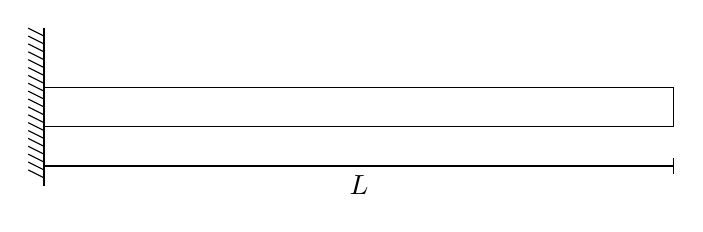
\begin{tikzpicture}[xscale=1, yscale=0.5]

        \draw (0,-0.5) rectangle (8, 0.5);
        \draw[|-|] (0, -1.5) -- (8, -1.5) node[midway, below]{$L$};

        \draw (0, -2) -- (0,  2);

        \foreach \y in {-1.8, -1.6, ..., 1.8}
        \draw (0, \y) -- ++(-0.2, +0.2);

    \end{tikzpicture}
    \caption{Aluminum beam with rectangular cross-section}
    \label{fig:beam}
\end{figure}

\begin{table}[H]
    \centering
    \begin{tabular}{lccc}
        \hline
        Parameter       & Symbol & Unit     & Value  \\
        \hline
        Length          & $L$    & $mm$     & $1200$ \\
        Thickness       & $h$    & $mm$     & $8$    \\
        Width           & $b$    & $mm$     & $40$   \\
        Density         & $\rho$ & $kg/m^3$ & $2700$ \\
        Young's modulus & $E$    & $GPa$    & $68$   \\
        \hline
    \end{tabular}
    \caption{Parameters of the cantilever beam}
    \label{tab:beam_parameters}
\end{table}

For this type of system/structure, considering zero axial-load, the standing wave equation governing its dynamics is:

\begin{equation}
    E I \frac{\partial^4 u}{\partial x^4} = - \rho A \frac{\partial^2 u}{\partial t^2}
\end{equation}

Which, when fully solved, leads to the following formulation of vertical displacement over time $w(x,t)$:

\begin{equation}
    w(x,t) = \left[A\cos(\gamma x) + B\sin(\gamma x) + C\cosh(\gamma x) + D\sinh(\gamma x)\right] \cos(\omega t + \phi)
\end{equation}

Where $\gamma^4 = \frac{m \omega^2}{EJ}$.

By applying the boundary conditions of the cantilever beam, we can find the natural frequencies (and successively also the mode shapes) of the system.
The equations that must be satisfied are:

\begin{equation}
    \begin{cases}
        w(0,t) = 0                                 \\
        \frac{\partial w}{\partial x}(0,t) = 0     \\
        \frac{\partial^2 w}{\partial x^2}(L,t) = 0 \\
        \frac{\partial^3 w}{\partial x^3}(L,t) = 0
    \end{cases}
\end{equation}

By highlighting the four unknowns $A$, $B$, $C$ and $D$, and rearranging the equations in a matrix form, we end up with a linear system as:

\begin{equation}
    [H(\omega)] z
    =
    \begin{bmatrix}
        1               & 0               & 1                & 0                \\
        0               & 1               & 0                & 1                \\
        -\cos(\gamma L) & -\sin(\gamma L) & +\cosh(\gamma L) & +\sinh(\gamma L) \\
        +\sin(\gamma L) & -\cos(\gamma L) & +\sinh(\gamma L) & +\cosh(\gamma L)
    \end{bmatrix}
    \begin{bmatrix}
        A \\
        B \\
        C \\
        D
    \end{bmatrix}
    =
    \begin{bmatrix}
        0 \\
        0 \\
        0 \\
        0
    \end{bmatrix}
    \label{eq:linear_system}
\end{equation}

\subsection{Computation of natural frequencies}
\label{subsec:natural_frequencies}

From theory, we know that the natural frequencies of a system can be computed by solving the following equation:

\begin{equation}
    det[H(\omega_n)] = 0
\end{equation}

Where $H(\omega_n)$ is the matrix as reported in Equation \ref{eq:linear_system} and $\omega_n$ is one of the natural frequencies.

By iterating over a given vector of frequencies, we can compute the value of the determinant of the matrix $H(\omega)$ and find the minimums, which correspond to the natural frequencies of the system.

The result of this computation is shown in Figure \ref{fig:natural_frequencies}.

\begin{figure}[H]
    \centering
    \includegraphics[width=\textwidth]{img/MATLAB/Part_A/H_module.png}
    \caption{Numerical search for natural frequencies of the system. Minimums value of $det[H(\omega)]$ are considered as natural frequencies.}
    \label{fig:natural_frequencies}
\end{figure}

\subsection{Computation of mode shapes}
\label{subsec:mode_shapes}

The mode shapes of the system can be computed again by considering the system of Equations \ref{eq:linear_system}.

In particular, given that to each natural frequency $\omega_n$ corresponds a mode shape, we can compute the mode shapes by solving the linear system for each natural frequency.
However, even if the system is exactly the same, it's important to understand that our goal now is to find the values of $A$, $B$, $C$ and $D$ that satisfy the system of equations, rather that finding the natural frequencies that cancel $H$.

In the end we will have a set of mode shapes, each one corresponding to a natural frequency of the system:

\begin{equation}
    H(\omega_{n, i}) z_i = 0
\end{equation}

By imposing the first component of the solution vector $z_i$ to be $A = 1$, we can find the other components of the solution vector.

\begin{equation}
    [H(\omega_{n, i})] z_i
    \rightarrow
    \hat z_i
    =
    \begin{bmatrix}
        B \\
        C \\
        D
    \end{bmatrix}
    =
    - \begin{bmatrix}
        1               & 0                & 1                \\
        -\sin(\gamma L) & +\cosh(\gamma L) & +\sinh(\gamma L) \\
        -\cos(\gamma L) & +\sinh(\gamma L) & +\cosh(\gamma L)
    \end{bmatrix}^{-1}
    \begin{bmatrix}
        0               \\
        -\cos(\gamma L) \\
        +\sin(\gamma L)
    \end{bmatrix}
    \label{eq:linear_system_for_mode_shapes}
\end{equation}

Once all the mode shapes coefficients ($A = 1$, $B$, $C$ and $D$) are computed, we can plot them with the indication of the associated natural frequency (see Figure \ref{fig:ideal_mode_shapes}).

\begin{figure}[H]
    \begin{minipage}[b]{0.45\textwidth}
        \centering
        \includegraphics[width=0.9\textwidth]{img/MATLAB/Part_A/Mode_shapes/mode_shape_01.png}
    \end{minipage}
    \hfill
    \begin{minipage}[b]{0.45\textwidth}
        \centering
        \includegraphics[width=0.9\textwidth]{img/MATLAB/Part_A/Mode_shapes/mode_shape_02.png}
    \end{minipage}
    \begin{minipage}[b]{0.45\textwidth}
        \centering
        \includegraphics[width=0.9\textwidth]{img/MATLAB/Part_A/Mode_shapes/mode_shape_03.png}
    \end{minipage}
    \hfill
    \begin{minipage}[b]{0.45\textwidth}
        \centering
        \includegraphics[width=0.9\textwidth]{img/MATLAB/Part_A/Mode_shapes/mode_shape_04.png}
    \end{minipage}
    \caption{Computed mode shapes starting from the ideal model of the cantilever beam.}
    \label{fig:ideal_mode_shapes}
\end{figure}

\section{Computation of FRFs}
\label{sec:computation_of_FRFs}

The computation of the FRFs is a crucial step in the analysis of the dynamic behavior of a structure.

The FRF is a complex-valued function that describes the steady-state response of a system to a sinusoidal excitation.
Even if the restriction over the shape of the excitation is quite severe, the FRF is a powerful tool to analyze the dynamic behavior of a system given that due to the linearity of the system, the response to a general excitation can be obtained by a linear combination of the responses to sinusoidal excitations (Fourier series).

By definition, the FRF is the ratio of the output to the input in the frequency domain.
For a linear time-invariant system, the FRF is a complex-valued function of the frequency, and it is defined as:

\begin{equation}
    H(\omega) = \frac{Y(\omega)}{X(\omega)}
\end{equation}

Where $H(\omega)$ is the FRF, $Y(\omega)$ is the Fourier transform of the output signal $y(t)$, and $X(\omega)$ is the Fourier transform of the input signal $x(t)$.

Moreover, to give a more practical definition, the FRF is the function that relates the output of a system considered at a specific coordinate to a sinusoidal input at a given coordinate.
If we then consider the system to be linear, time-invariant, and with a single input $@x_k$ and a single output $@x_j$, than the FRF can be defined as:

\begin{equation}
    H_{j,k}(\Omega) = \sum_{i=1}^{n} \frac{\Phi_i(x_j) \Phi_i(x_k) / m_i}{-\Omega^2 + 2\xi_i \omega_i \Omega i + \omega_i^2}
    \label{eq:FRF}
\end{equation}

Where, all the entities of Equation \ref{eq:FRF} are defined in Table \ref{tab:FRF_entities}.

\begin{table}[H]
    \centering
    \begin{tabular}{cl}
        \hline
        Parameter     & Description                                         \\
        \hline
        $\Phi_i(x^*)$ & Mode shape of the $i^{th}$ mode at coordinate $x^*$ \\
        $m_i$         & Equivalent mass of the $i^{th}$ mode                \\
        $\xi_i$       & Damping ratio of the $i^{th}$ mode                  \\
        $\omega_i$    & Natural frequency associated to the $i^{th}$ mode   \\
        $\Omega$      & Frequency of the sinusoidal excitation              \\
        \hline
    \end{tabular}
    \caption{Entities explanation for Equation \ref{eq:FRF}}
    \label{tab:FRF_entities}
\end{table}

As we can notice, among the entities of Equation \ref{eq:FRF}, at the moment we are only missing the equivalent mass $m_i$ and the damping ratio $\xi_i$.

The equivalent mass $m_i$ is a fictitious value that represents the amount of mass of the system that is effectively moving in the $i^{th}$ mode, weighted by the mode shape.
From this definition, we get:

\begin{equation}
    m_i = \int_{0}^{L} \rho A \Phi_i^2(x) dx
\end{equation}

For the damping ratio $\xi_i$, we can either use the Rayleigh damping model or the modal damping model.
However, since we are not dealing with a discretized system, but rather with a continuous one, for the sake of simplicity we will assume the damping ratio to be $\xi_i = \frac{c_i}{2 \sqrt{m_i k_i}} = 0.01$.

By doing so, we can compute the FRFs for the system at hand, and we can analyze the dynamic behavior of the structure.

\subsection{FRFs of the system due to a single point force}
\label{subsec:FRFs_of_the_system_due_to_a_single_point_force}

Once the FRFs function is defined, we can think of interrogate the structure to see how it reacts due to a single point force applied at a specific coordinate.

In particular, we can consider a sinusoidal force applied at coordinate $x_k = 0.9m$ and see how the structure reacts at a set of coordinates $x_j = [0.2 \quad 0.4 \quad 0.6 \quad 0.8 \quad 1.0 \quad 1.2]m$.
A graphical representation of the considered situation can be seen in Figure \ref{fig:beam_single_point_force}.

\begin{figure}[H]
    \centering
    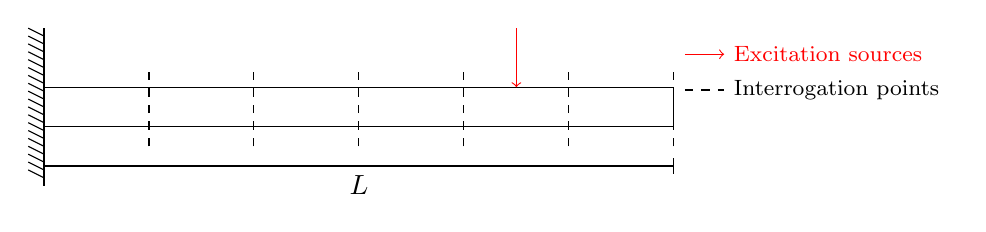
\begin{tikzpicture}[xscale=1, yscale=0.5]

        \draw (0,-0.5) rectangle (8, 0.5);
        \draw[|-|] (0, -1.5) -- (8, -1.5) node[midway, below]{$L$};

        \draw (0, -2) -- (0,  2);

        \foreach \y in {-1.8, -1.6, ..., 1.8}
        \draw (0, \y) -- ++(-0.2, +0.2);

        \foreach \x in {0.2, 0.4, ..., 1.2}
        \draw[dashed] (\x * 8/1.2, -1.0) -- ++(0.0, +2.0);

        \draw[<-, red] (0.9 * 8/1.2, 0.5) -- ++(0.0, +1.5);

        % Add legend
        \node [matrix, font = \footnotesize, below right, row sep = 0cm] at (current bounding box.north east)
        {
            \draw[->, red] (0, 0) -- ++(0.5, 0) node[right, red] {Excitation sources}; \\
            \draw[dashed, black] (0, 0) -- ++(0.5, 0) node[right, black] {Interrogation points}; \\
        };

    \end{tikzpicture}
    \caption{Analyzed situation: single input, multiple outputs}
    \label{fig:beam_single_point_force}
\end{figure}

Since we are now considering $6$ different coordinates, we will have $6$ different FRFs, each one describing the response of the structure at a specific coordinate due to the excitation $f(t) = F_0 \sin(\Omega t) = 1 \sin(\Omega t)$.

By doing so, we obtain the module and phase plots reported in Figure \ref{fig:FRFs_single_point_force}.

\begin{figure}[H]
    \centering
    \includegraphics[width=\textwidth]{img/MATLAB/Part_A/Experimental_FRF_SIMO.png}
    \caption{FRFs of the system due to a single point force. Each color in the plot represents the FRF of the structure at a specific output coordinate.}
    \label{fig:FRFs_single_point_force}
\end{figure}

\subsection{FRFs of the system due to a multiple point force}
\label{subsec:FRFs_of_the_system_due_to_multiple_point_force}

The next step is to observe the behavior of the structure when multiple forces are applied to it.

As we have said in the previous section, even if the FRF given information about a single input and a single output, we can still use it to understand how the structure behaves when multiple forces are applied to it and study the structural response at different coordinates.

For the sake of simplicity, we will consider a structure with $2$ excitation points at $x_k = [0.3 0.9]m$ and $3$ output points at $x_j = [0.2 0.8 1.2]m$.

A graphical representation of the considered situation can be seen in Figure \ref{fig:beam_multi_point_force}.

\begin{figure}[H]
    \centering
    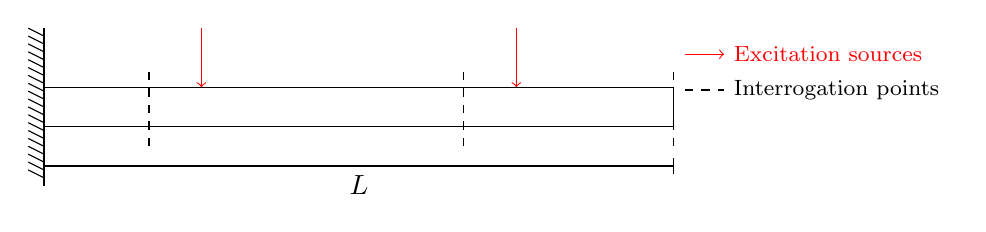
\begin{tikzpicture}[xscale=1, yscale=0.5]

        \draw (0,-0.5) rectangle (8, 0.5);
        \draw[|-|] (0, -1.5) -- (8, -1.5) node[midway, below]{$L$};

        \draw (0, -2) -- (0,  2);

        \foreach \y in {-1.8, -1.6, ..., 1.8}
        \draw (0, \y) -- ++(-0.2, +0.2);

        \foreach \x in {0.2, 0.8, 1.2}
        \draw[dashed] (\x * 8/1.2, -1.0) -- ++(0.0, +2.0);

        \foreach \x in {0.3, 0.9}
        \draw[<-, red] (\x * 8/1.2, 0.5) -- ++(0.0, +1.5);

        % Add legend
        \node [matrix, font = \footnotesize, below right, row sep = 0cm] at (current bounding box.north east)
        {
            \draw[->, red] (0, 0) -- ++(0.5, 0) node[right, red] {Excitation sources}; \\
            \draw[dashed, black] (0, 0) -- ++(0.5, 0) node[right, black] {Interrogation points}; \\
        };

    \end{tikzpicture}
    \caption{Analyzed situation: multiple inputs, multiple outputs}
    \label{fig:beam_multi_point_force}
\end{figure}

Similar reasoning as before can be done about the expected result of this type of analysis in terms of number of FRFs to be computed and the information that can be extracted from them.

Moreover, given that we are now dealing with a multi-input system, the actual displacement of the structure at a specific coordinate will be the result of the superposition of the displacements due to each excitation force.

Before proceeding with the visualization of the actual FRFs, it's important to stress that what we are actually "superposing" are the complex FRFs, not only their modules.
This means that the phase information is also taken into account when computing the total response of the structure.
But also remember that the phase information is also dependent on the phase of the input force, so it's important to keep track of it when analyzing the results.

To better understand this aspect, we can move on a complex plane and consider the output of a generic system due to two different input forces $F_1 = F_{1,0} \sin(\omega_1 t + \phi_1)$ and $F_2 = F_{2,0} \sin(\omega_2 t + \phi_2)$.

\begin{figure}[H]
    \centering
    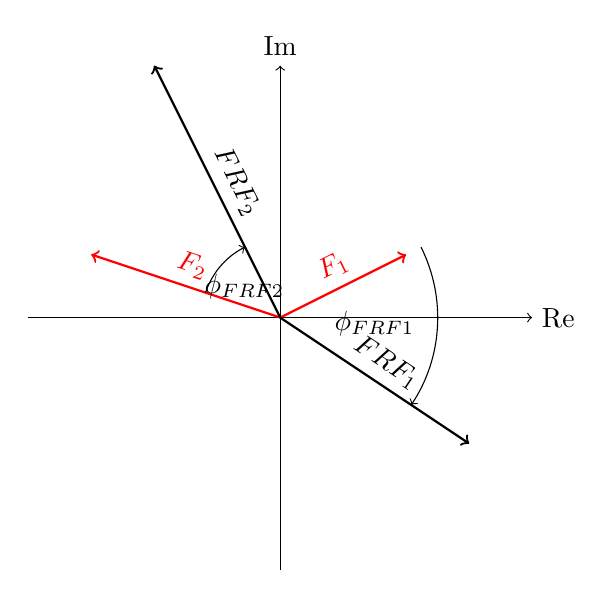
\begin{tikzpicture}[scale=0.8]

        \coordinate (O) at (0, 0);
        \coordinate (A) at (2, 1);
        \coordinate (B) at (-3, 1);
        \coordinate (C) at (3, -2);
        \coordinate (D) at (-2, 4);

        \draw[->] (-4,0) -- (4,0) node[right] {Re};
        \draw[->] (0,-4) -- (0,4) node[above] {Im};

        \draw[->, thick, red] (O) -- (A) node[midway, above, sloped] {$F_1$};
        \draw[->, thick, red] (O) -- (B) node[midway, above, sloped] {$F_2$};
        \draw[->, thick] (O) -- (C) node[midway, above, sloped] {$FRF_1$};
        \draw[->, thick] (O) -- (D) node[midway, above, sloped] {$FRF_2$};

        \pic [draw, <-, "$\phi_{FRF1}$", angle radius = 2cm] {angle = C--O--A};
        \pic [draw, <-, "$\phi_{FRF2}$", angle radius = 1cm] {angle = D--O--B};

    \end{tikzpicture}
    \hfill
    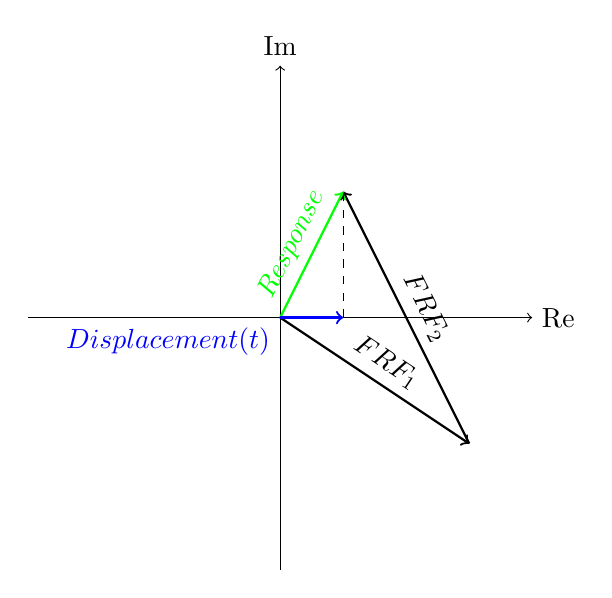
\begin{tikzpicture}[scale=0.8]

        \coordinate (O) at (0, 0);
        \coordinate (A) at (2, 1);
        \coordinate (B) at (-3, 1);
        \coordinate (C) at (3, -2);
        \coordinate (D) at (-2, 4);

        \draw[->] (-4,0) -- (4,0) node[right] {Re};
        \draw[->] (0,-4) -- (0,4) node[above] {Im};

        \draw[->, thick] (O) -- (C) node[midway, above, sloped] {$FRF_1$};
        \draw[->, thick] (C) -- ++(D) node[midway, above, sloped] {$FRF_2$};

        \draw[->, thick, green] (O) -- (1, 2) node[midway, above, sloped] {$Response$};
        \draw[dashed] (1, 0) -- (1, 2);
        \draw[->, thick, blue] (O) -- (1, 0) node[below left] at (O) {$\text{Displacement}(t)$};



    \end{tikzpicture}
    \caption{Complex plane representation of the FRFs of the system due to multiple input forces and the actual displacement of the output/interrogation point.}
    \label{fig:complex_plane_representation}
\end{figure}

As is clearly see in Figure \ref{fig:complex_plane_representation}, the actual displacement of the output point can in some cases (or better for some period of time) be definitely lower than the sum of just the absolute modules of the FRFs.

If we came back and considering again the situation represented in Figure \ref{fig:beam_multi_point_force}, we obtain the module and phase plots reported in Figure \ref{fig:FRFs_multi_point_force}.

\begin{figure}[H]
    \centering
    \includegraphics[width=\textwidth]{img/MATLAB/Part_A/Experimental_FRF_MIMO.png}
    \caption{FRFs of the system due to a couple of point force. Each color in the plot represents the FRF of the structure at a specific output coordinate.}
    \label{fig:FRFs_multi_point_force}
\end{figure}

\section{Parameters identification}
\label{sec:parameters_identification}

In this section, we are going to explain the procedure followed to identify the parameters of the system starting from the FRFs obtained in the previous section.
Basically we are going to simulate an `Operational Modal Analysis' (OMA), even if in this case we already have the exact model of the system.

In particular, we know that for a multi degree-of-freedom system, with lightly damped modes and in particular in case of well distinguished peaks, the FRF can be approximated around a given natural frequency $\omega_n$ as:

\begin{equation}
    H{j, k}^{NUM}(\Omega) = \frac{A_{j, k}^(i)}{-\Omega^2 + 2 \xi_i \omega_i \Omega + \omega_i^2} + \frac{R_{j, k}^L}{\Omega^2} + R_{j, k}^{H} \quad \text{for} \quad \Omega_{min} \leq \omega_i \leq \Omega_{max}
    \label{eq:FRF_approximation}
\end{equation}

As we can see, the FRF is approximated as a sum of three terms: a second order term, a low frequency term and a high frequency term.
The second order term is the one that we are interested in, since it is the one that contains the information about the natural frequency and the damping ratio of the system.
However, if the peaks are not well distinguished, the low and high frequency terms can interfere with the second order term and became non-negligible in the approximation.

In the following, a common procedure is explained to identify all the unknown parameters of $H{j, k}^{NUM}(\Omega)$, once the experimental FRFs are available.
In particular, we will see how to identify the natural frequencies $\omega_i^{NUM}$, the damping ratios $\xi_i^{NUM}$, and the gains $A_{j, k}^{NUM}$, $R_{j, k}^L$ and $R_{j, k}^H$, using minimization techniques.


\subsection{Procedure}
\label{subsec:procedure}

Many of the following steps are based on the assumption that the frequencies vector defining the FRFs, has a higher enough resolution to properly address the following procedure.
In case of a low resolution, the frequencies vector should be at least interpolated in order to obtain a more fine grid over the frequency range of interest.

All the following steps, must be repeated for each natural frequency $\omega_i$ of the system.

\paragraph{Natural frequencies}

The first step is to identify the value of the natural frequency $\omega_i^{NUM}$ of the system.

This can be done by looking at the peaks of the FRFs.
If we have many FRFs at our disposal (for example, we have many sensors or we have performed many tests), we can average the FRFs in order to reduce the noise and obtain a more reliable result.
Remember that the natural frequency identified has to be the same for all the FRFs.

\paragraph{Damping ratios}

The second step is to identify the value of the damping ratio $\xi_i^{NUM}$ of the system.

For this purpose, we can use both the `phase derivative' method or the `half power bandwidth' method (also known as `peak picking' method).

For this assignment, we decided to use the `phase derivative' method, given that the experimental FRFs have a fine enough grid of frequencies.

By looking at the phase of the FRF evaluated at the natural frequency $\omega_i$, we observe that the slope of the phase can be directly related to the damping ratio $\xi_i$.
In particular:

\begin{equation}
    \frac{\partial \angle H_{j, k}(\Omega)}{\partial \Omega} \biggl|_{\Omega = \omega_i} = - \frac{1}{\xi_i \omega_i}
    \label{eq:phase_derivative}
\end{equation}

Based on this relation, we can isolate the damping ratio $\xi_i$ and obtain its value numerically, computing the derivative of the phase of the FRF evaluated at the natural frequency $\omega_i$ using a finite difference method.

\begin{equation}
    \xi_i^{NUM} = - \frac{1}{\omega_i^{NUM} \cdot \frac{\Delta \angle G_{i,k}^{NUM}(\omega_i^{NUM})}{\Delta \omega}}
\end{equation}

\paragraph{Gain $A_{j, k}^{NUM}$}

The third step is to identify the value of the gain $A_{j, k}^{NUM}$ of the system.

This can be done by looking at the magnitude of the FRFs evaluated at the natural frequency $\omega_i$.
In particular, we can obtain the value of the gain $A_{j, k}^{NUM}$ numerically as:

\begin{equation}
    A_{j, k}^{NUM} = -2i \left| G_{j, k}^{EXP}(\omega_i^{NUM}) \right| \omega_i^2 \xi_i^{NUM}
\end{equation}

However, in order to reduce the disturbances effects coming from the low and high frequency terms, we decided to use a more robust method to identify the gain $A_{j, k}^{NUM}$, relying on just the imaginary part of the FRF evaluated at the natural frequency $\omega_i$:

\begin{equation}
    A_{j, k}^{NUM} = - Im\left[2\left| G_{j, k}^{EXP}(\omega_i^{NUM}) \right| \omega_i^2 \xi_i^{NUM}\right]
\end{equation}

\paragraph{Final minimization algorithm}

Finally, we can proceed with the minimization of the error between the experimental FRFs and the model FRFs, in order to identify the `exact' values of all the parameters of the system, since the previous steps are only needed as a first approximation.

To do so, we define the error function as:

\begin{equation}
    \epsilon = \sum_{j, k, \Omega} \left| H_{j, k}^{NUM}(\Omega) - H_{j, k}^{EXP}(\Omega) \right|^2
    \label{eq:error_function}
\end{equation}

Which we can think of as the sum of the squared differences between the experimental FRFs and the numerical FRFs evaluated at all the considered frequencies around the analyzed natural frequency $\omega_i$.

In order to minimize the error function, we can use a minimization algorithm, such as the `Levenberg-Marquardt' algorithm, which is a combination of the `Gauss-Newton' algorithm and the `Steepest Descent' algorithm.
This algorithm is particularly useful in case of non-linear least squares problems, such as the one we are facing.

In \texttt{MATLAB}, the `Levenberg-Marquardt' algorithm is implemented in the function \texttt{lsqnonlin}.

\subsection{Parameters identification results}
\label{subsec:parameters_identification_results}

Once the previously explained procedure has been applied to all the natural frequencies of the system (consider for each one, every experimental FRFs at our disposal), we can reassemble the identified parameters so to compute the numerical FRFs of the system.

In the following figures, the result obtained considering the FRF relative to an input in $x_k = 1.0m$ and an output in $y_j = 0.6m$ is shown.

\begin{center}
    \huge{Plot to be replaced with the correct one.}
\end{center}

\begin{figure}[H]
    \centering
    \includegraphics[width=\textwidth]{img/MATLAB/Part_A/Comparison_FRF_couple_1_6.png}
    \caption{FRF identification for $x_k = 1.0m$ and $y_j = 0.6m$}
    \label{fig:FRF_identification}
\end{figure}

\begin{center}
    \huge{Plot to be replaced with the 4 zooms over the 4 peaks.}
\end{center}

\begin{figure}[H]
    \begin{minipage}[b]{0.45\textwidth}
        \centering
        \includegraphics[width=\textwidth]{img/MATLAB/Part_A/Mode_shapes/mode_shape_01.png}
    \end{minipage}
    \hfill
    \begin{minipage}[b]{0.45\textwidth}
        \centering
        \includegraphics[width=\textwidth]{img/MATLAB/Part_A/Mode_shapes/mode_shape_02.png}
    \end{minipage}
    \begin{minipage}[b]{0.45\textwidth}
        \centering
        \includegraphics[width=\textwidth]{img/MATLAB/Part_A/Mode_shapes/mode_shape_03.png}
    \end{minipage}
    \hfill
    \begin{minipage}[b]{0.45\textwidth}
        \centering
        \includegraphics[width=\textwidth]{img/MATLAB/Part_A/Mode_shapes/mode_shape_04.png}
    \end{minipage}
    \caption{Zoom over the peaks of the FRF identification for $x_k = 1.0m$ and $y_j = 0.6m$}
    \label{fig:FRF_identification_zoom}
\end{figure}


\section{Final results (mode shapes comparison)}
\label{sec:final_results_A}

Even if the comparison between the experimental FRFs and the numerical FRFs in the complex plane is a good way to validate the identified parameters, it is also useful to compare the mode shapes obtained from the experimental data with the ones obtained from the numerical model.

In the following figures, the experimental (from flexible body theory) and numerical mode shapes are compared for the first 4 modes of the system.
% In particular, even if in theory the mode shapes are characteristic of the structure per se, the numerical model is not able to capture exactly the same shape for every set of input-output points.

% To be consistent with the previously shown FRF figures, we are now going to represent the experimental mode shapes in blue, and the numerical mode shapes computed considering an input in $x_k = 1.0m$ and an output in $y_j = 0.6m$ is shown.

\begin{figure}[H]
    \begin{minipage}[b]{0.45\textwidth}
        \centering
        \includegraphics[width=\textwidth]{img/MATLAB/Part_A/Comparison_ModeShape_01.png}
    \end{minipage}
    \hfill
    \begin{minipage}[b]{0.45\textwidth}
        \centering
        \includegraphics[width=\textwidth]{img/MATLAB/Part_A/Comparison_ModeShape_02.png}
    \end{minipage}
    \begin{minipage}[b]{0.45\textwidth}
        \centering
        \includegraphics[width=\textwidth]{img/MATLAB/Part_A/Comparison_ModeShape_03.png}
    \end{minipage}
    \hfill
    \begin{minipage}[b]{0.45\textwidth}
        \centering
        \includegraphics[width=\textwidth]{img/MATLAB/Part_A/Comparison_ModeShape_04.png}
    \end{minipage}
    \caption{Comparison between experimental and numerical mode shapes}
    \label{fig:Mode_shapes_comparison}
\end{figure}

Numerically speaking, we can also report the relative error between the experimental and numerical natural frequencies, defined as follows:

\begin{equation}
    \text{Relative error} = \frac{\sum_{i=1}^{N} \left| \omega_{\text{exp},i} - \omega_{\text{num},i} \right|}{\sum_{i=1}^{N} \left| \omega_{\text{exp},i} \right|} \%
\end{equation}

Where $\omega_{\text{exp},i}$ and $\omega_{\text{num},i}$ are the $i$-th experimental and numerical natural frequencies, respectively.

The relative error for the first 4 natural frequencies of the system is reported in the following table.

\begin{table}[H]
    \centering
    \begin{tabular}{lccc}
        \hline
        Mode & Experimental [rad/s] & Numerical [rad/s] & Relative error [\%] \\
        \hline
        1    & 28.2767              & 28.2524           & 0.0859              \\
        2    & 177.3053             & 177.2344          & 0.0400              \\
        3    & 496.5177             & 496.3996          & 0.0238              \\
        4    & 973.0323             & 973.0560          & -0.0024             \\
        \hline
    \end{tabular}
    \caption{Relative error between experimental (in this case coming the flexible body theory) and numerical natural frequencies.}
    \label{tab:Relative_error_frequencies}
\end{table}


\clearpage
\section{Requests (Part B)}
\label{sec:requests_part_B}

The requests for `Assignment 1 (Part B)' are the followings:

\begin{itemize}
    \item Apply the procedure developed within Part A to the provided experimental data, to identify the modal parameters (natural frequencies, damping ratios and mode shapes) of the first two axial modes.
    \item Check the quality of the identification comparing the identified FRFs and the experimental ones.
    \item Plot a diagram showing the identified mode shapes with the indication of the corresponding natural frequencies and damping ratios.
\end{itemize}

\section{Data Analysis}
\label{sec:data_analysis}

In this section, the data collected during the experimental campaign are analyzed.
The data are processed exactly as described in the previous section (see Section \ref{sec:parameters_identification}), and the identified parameters are used to compute the numerical FRFs and the mode shapes of the system.

In particular, by plotting the given data (which are the experimental FRFs comping from impact test performed on a rail wheel and sampled in different angular position), we can clearly see that multiple peaks are present (see Figure \ref{fig:FRFs_part_B}).
However, this study will be focused on the first two peaks only, given that considering the real system from which data are acquired, those are the ones of interest.

\begin{figure}[H]
    \centering
    \includegraphics[width=\textwidth]{img/MATLAB/Part_B/Experimental_data.png}
    \caption{FRFs and coherence functions of the system.}
    \label{fig:FRFs_part_B}
\end{figure}


\subsection{First peak}
\label{subsec:first_peak}

Modal parameters analysis applied to the first peak of the FRFs allows us to identify the natural frequency and the damping ratio of the first mode.
The identified parameters are reported in Table \ref{tab:first_peak}.

\begin{table}[H]
    \centering
    \begin{tabular}{lc}
        \hline
        $frequency_i [Hz]$ & ?? \\
        \hline
        $\xi_i [\%]$       & ?? \\
        \hline
    \end{tabular}
    \caption{First peak modal parameters.}
    \label{tab:first_peak}
\end{table}

From a graphical point of view, the experimental and numerical FRFs are compared in Figure \ref{fig:first_peak}.

\begin{center}
    \huge{Plot to be replaced with the correct one.}
\end{center}

\begin{figure}[H]
    \centering
    \includegraphics[width=\textwidth]{img/MATLAB/Part_B/Comparison_FRF_1.png}
    \caption{First peak FRFs comparison.}
    \label{fig:first_peak}
\end{figure}



\subsection{Second peak}
\label{subsec:second_peak}

Modal parameters analysis applied to the second peak of the FRFs allows us to identify the natural frequency and the damping ratio of the second mode.
The identified parameters are reported in Table \ref{tab:second_peak}.

\begin{table}[H]
    \centering
    \begin{tabular}{lc}
        \hline
        $frequency_i [Hz]$ & ?? \\
        \hline
        $\xi_i [\%]$       & ?? \\
        \hline
    \end{tabular}
    \caption{Second peak modal parameters.}
    \label{tab:second_peak}
\end{table}

From a graphical point of view, the experimental and numerical FRFs are compared in Figure \ref{fig:second_peak}.

\begin{center}
    \huge{Plot to be replaced with the correct one.}
\end{center}

\begin{figure}[H]
    \centering
    \includegraphics[width=\textwidth]{img/MATLAB/Part_B/Comparison_FRF_1.png}
    \caption{Second peak FRFs comparison.}
    \label{fig:second_peak}
\end{figure}


\begin{figure}[H]
    \centering
    \begin{minipage}{0.45\textwidth}
        \centering
        \includegraphics[width=\textwidth]{img/MATLAB/Part_B/Comparison_FRF_1_zoom_peak_01.png}
        \caption{First peak FRFs comparison.}
        \label{fig:first_peak}
    \end{minipage}
    \hfill
    \begin{minipage}{0.45\textwidth}
        \centering
        \includegraphics[width=\textwidth]{img/MATLAB/Part_B/Comparison_FRF_1_zoom_peak_02.png}
        \caption{Second peak FRFs comparison.}
        \label{fig:second_peak}
    \end{minipage}
\end{figure}
\section{Final Results (mode shapes visualization)}
\label{sec:final_results_B}

In this section, the identified mode shapes identified from the experimental data are reported.

\begin{figure}[H]
    \centering
    \includegraphics[width=0.45\textwidth]{img/MATLAB/Part_B/ModeShape_01.png}
    \hfill
    \includegraphics[width=0.45\textwidth]{img/MATLAB/Part_B/ModeShape_02.png}
    \caption{Identified (numerically) first two mode shapes of the system.}
    \label{fig:mode_shapes}
\end{figure}

Notice that those graph must be interpreted as axial displacements with respect to the un-deformed system.
Basically, the more the colored line are far from the black dashed line, the more the system is axially deformed in that region.
Moreover, the position of the colored lines with respect to the black dashed line (external or internal) indicates the direction of the deformation with respect to the un-deformed plane of the system.

The first mode shape (Figure \ref{fig:mode_shapes}, left) can also be visualized in a 3D way that to a FEA simulation performed in \cite{FEM_rail_wheel}.

\begin{figure}[H]
    \centering
    \includegraphics[width=0.7\textwidth]{img/wheel-FEM-first-mode-shape.png}
    \caption{First mode shape of the system visualized in a 3D way. Credit to \cite{FEM_rail_wheel}.}
    \label{fig:mode_shape_3D}
\end{figure}

As a final remark, we report in Table \ref{tab:mode_shapes_parameters} the identified parameters for the first two mode shapes of the system.

\begin{table}[H]
    \centering
    \begin{tabular}{lcc}
        \hline
        Mode & Frequency [Hz] & Damping ratio [\%] \\
        \hline
        1    & 667.324        & 0.75 \%            \\
        2    & 1625.312       & 0.59 \%            \\
        \hline
    \end{tabular}
    \caption{Identified parameters for the first two mode shapes of the system.}
    \label{tab:mode_shapes_parameters}
\end{table}



% \clearpage
\vfill
\bibliographystyle{plain}
\bibliography{refereces.bib}

\end{document}
